% !TEX encoding = UTF-8
% !TEX program = xelatex
\documentclass[12pt,a4paper]{article}
\usepackage[paperwidth=210mm, paperheight=297mm, left=0.75in, right=0.75in, bottom=1in, top=1in]{geometry}
%\usepackage{geometry}
\usepackage{polyglossia}
\setdefaultlanguage[babelshorthands]{italian}
\usepackage{fontspec}
%\usepackage{cite}
\usepackage{graphicx}
%\usepackage[fixlanguage]{babelbib}
%\selectbiblanguage{italian}
\usepackage{blindtext}
\usepackage{wrapfig}

\frenchspacing
\makeindex

\begin{document}
\title{\vspace{-70pt}ARGOS}
\author{Nicola Ballista}
\date{}
\maketitle
\pagestyle{empty}
\thispagestyle{empty}

% aggiungere asterischi
% cambiare nome e autore
% spostare figura
% pack

\def\nomedelsatellite{ARGOS}
\def\autore{Ballista Nicola}

\section*{Storia}
\label{storia}
\begin{wrapfigure}{r}{0.35\textwidth}
  \vspace{-10pt}
  \begin{center}
    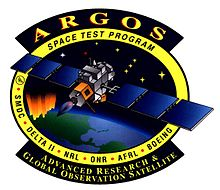
\includegraphics[width=0.30\textwidth]{satellite}
  \end{center}
  \vspace{-20pt}
  %\caption{A gull}
\end{wrapfigure}
\textbf{Argos} è un satellite basato su un sistema che raccoglie, elabora e diffonde \emph{dati ambientali} da piattaforme fisse e mobili in tutto il mondo. Ciò che rende Argos unico è la capacità di individuare geograficamente la fonte dei dati ovunque sulla Terra utilizzando l'\textbf{effetto Doppler}.
Argos è stata fondata nel 1978 e da allora, ha fornito i dati per la ricerca ambientale e le comunità di protezione che, in molti casi, era altrimenti irrealizzabile. Il sistema è pienamente provato e altamente affidabile. Molte remote stazioni meteorologiche automatiche riportano i loro dati via Argos. Argos è un componente chiave di molti programmi di ricerca a livello mondiale tra cui: programma Tropical Atmosphere Ocean-Global (TOGA), Tagging of Pacific pelagici (TOPP), World Ocean Circulation Experiment (WOCE), Argo e altri.

\section*{Osservazioni}
\label{osservazioni}

Dalla fine degli anni 1980 gli Argos trasmettitori sono stati regolarmente distribuiti su un gran numero di \emph{mammiferi marini} e tartarughe di mare e continua a rappresentare lo strumento più importante per il monitoraggio dei movimenti a lunga distanza di specie sia costiere che oceaniche. Mediante il caricamento di dati provenienti, per esempio, da trasduttori di pressione, è stato possibile ottenere anche un patrimonio di conoscenze circa l'immersione e il comportamento alimentare di animali in natura.

\section*{Curiosità}
\label{curiosit}

Argos è stato sviluppato nell'ambito di un \emph{Memorandum of Understanding} (MOU) tra il Centro Nazionale di Studi Spaziali (CNES, l'agenzia spaziale francese), la National Aeronautics and Space Administration (NASA, USA) e la National Oceanic and Atmospheric Administration (NOAA, USA ).


\end{document}